\chapter{Gamma-Ray Astronomy} \label{sec:02_astronomy}

\autoref{sec:01_PWN_chapter} discussed how PWNe like \mbox{HESS\,J1825-137} accelerate cosmic rays up to $\TeV$ energies and how gamma rays can be used as alternative messengers. To study accelerators like \mbox{HESS\,J1825-137}, astronomers require instruments that are capable of observing gamma rays up to $\TeV$ energies.
\newpar 
Upon reaching the Earth atmosphere, gamma rays produce air showers comprising of billions of secondary particles and photons. Astronomers in the early 20th century placed Geiger counters on balloons to detect gamma rays at high altitude \citep{hess1912observations}. Now, satellites like \textit{Fermi}-LAT are used to observe gamma rays less than $\approx 0.1\,\TeV$ before they enter the atmosphere \citep{2010RPPh...73g4901M}. Alternatively, ground-based observatories analyse the air shower itself to reconstruct information about the original gamma ray. This is a method used by the High Energy Stereoscopic System (H.E.S.S.) to study $\TeV$ gamma-ray sources like \mbox{HESS\,J1825-137}.
\newpar 
This section will provide a brief overview of how gamma rays interact with the atmosphere and the techniques used to observe the subsequent shower of particles. Finally, there will be a description of the gamma-ray observatories whose data products were utilised in this thesis.% in particular the High Energy Stereoscopic System (H.E.S.S.).

\section{Air Showers}

The presence of molecules in the atmosphere provides a target for gamma rays and cosmic-ray protons to interact and produce lower energy particles (electrons, positrons, pions). The daughter particles then go on to decay or interact with the atmosphere to produce even lower energy particles. This process cascades to form an air shower which is shown in \autoref{fig:chapter_2_air_shower_em} and \autoref{fig:chapter_2_air_shower_hadron}.
\newpar 
The morphology and structure of the air shower is dependent on the atmosphere. Atmospheric depth is defined to be the attitudinal integral of atmospheric density above height $h$ \citep{alma9924446790001811}:

\begin{equation}
    \begin{aligned}
    X&=\int_{h}^\infty \rho\qty(h')\dd{h'}\text{ ,}
    \end{aligned}
\end{equation}
\noindent with the units of atmospheric depth being $\grampercentimetresquared$. Atmospheric depth is a proxy for the amount of material above height $h$. For a constant temperature, the relationship between height and atmospheric depth becomes:

\begin{equation}
    \begin{aligned}
    X=X_0\exp(-h/h_0)\text{ ,}
    \end{aligned}
\end{equation}
where $h_0$ is the scale height of the atmosphere and $X_0=1030\,\grampercentimetresquared$ is the atmospheric depth at sea level. 

\subsection{Gamma-Ray Air Showers} \label{sec:05_air_shower_gamma_ray}
To produce an electron-positron pair, a gamma ray must be in the vicinity of a nucleus to conserve both momentum and energy. When a gamma ray above a few $\GeV$ enters the atmosphere, the presence of atmospheric nuclei allows pair production to occur:
\begin{equation}
    \begin{aligned}
    \gamma + Z &\rightarrow e^- + e^+
    \end{aligned}
\end{equation}
\noindent where the daughter electron and positron each have kinetic energy:
\begin{equation}
    \begin{aligned}
    E_{e^\pm}&\approx \half\qty(E_\gamma-2m_ec^2)\text{ ,}
    \end{aligned} \label{eq:05_gamma_astrom_pair_condition}
\end{equation}
\noindent with $E_\gamma$ being the energy of the original gamma ray. Hence, the original gamma ray must have a threshold energy of twice the rest mas of the electron ($m_ec^2=511\,\keV$) to undergo pair production.
\newpar
Electrons and positrons interact with atmospheric nucleii through Bremsstrahlung interactions (see \autoref{sec:chapter_1_leptonic_gre}), resulting in the production of photons:

\begin{equation}
    \begin{aligned}
    e_\pm' + Z & \rightarrow e_{\pm} + Z + \gamma
    \end{aligned}
\end{equation}
\noindent with a cross section, $\dd{\sigma}_\text{brem}$, described by \autoref{eq:chapter_1_non_thermal_brem_cross_section} . The distance that an electron/positron travels before radiating a photon through Bremsstrahlung interactions is given by \citep{MATTHEWS2005387}:

\begin{equation}
    \begin{aligned}
    d=\lambda_r \ln 2\text{ ,}
    \end{aligned}
\end{equation}
\noindent where the radiation length, $\lambda_r$, is characteristic to a material and relates to the energy loss of high-energy particles as it transverses through a medium.
\newpar 
Positrons can also annihilate with atmospheric electrons to produce two photons:

\begin{equation}
    \begin{aligned}
    e^- + e^+&\rightarrow \gamma + \gamma
    \end{aligned}
\end{equation}
with each daughter photon having threshold energy $E_\text{thr}\geq m_ec^2$. If the daughter photons have energy greater than twice the rest mass of an electron (\autoref{eq:05_gamma_astrom_pair_condition}), they can undergo electron-positron production. The cross section for electron-positron production, $\sigma_\text{pair}$, can be given in terms of the cross section for Bremsstrahlung interactions, $\sigma_\text{br}$, by:

\begin{equation}
    \begin{aligned}
    \sigma_\text{pair}\qty(E_e,_E\gamma)&=\sigma_\text{br}\qty(E_e,E_\gamma)\frac{E_e^2}{E_\gamma^2}\approx \frac{7}{9}\sigma_\text{br}\qty(E_e,E_\gamma)\text{ ,}
    \end{aligned} \label{eq:chapter_2_pair_prod_cs}
\end{equation}
where $k$ is the energy of the resulting photons.
\begin{SCfigure}[1][h!]
    % \centering
    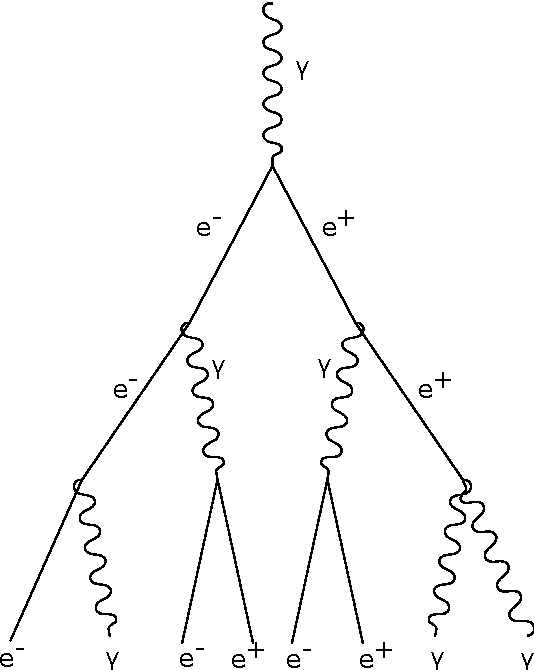
\includegraphics[width=0.5\textwidth]{05_Astronomy/Images/air_shower/gamma_ray.pdf}
    \caption{Heitler's model of the formation of an air shower triggered by a gamma ray \citep{1954qtr..book.....H}. The gamma ray undergoes pair production to produce an electron and positron. In turn, the electron/positron undergo Bremsstrahlung interactions and/or electron-positron annihilation to produce photons. This process cascades into the air shower.}
    \label{fig:chapter_2_air_shower_em}
\end{SCfigure}
\newpar 
Heitler's model of electromagnetic air showers (see \autoref{fig:chapter_2_air_shower_em}) provides a method to model the development of the electromagnetic shower \citep{1934RSPSA.146...83B}. It assumes that the radiation length for both pair production and Bremsstrahlung interactions are identical due to a similar cross section. Therefore, the atmospheric depth of the air shower after $n$ interactions is:

\begin{equation}
    \begin{aligned}
    X=nd=n\lambda_r\ln 2\text{ .}
    \end{aligned} \label{eq:chapter_2_gas_depth}
\end{equation}
\noindent The number of particles (electrons, positrons and photons) in the air shower after $n$ interactions is given by \citep{MATTHEWS2005387}:
\begin{equation}
    \begin{aligned}
    N&=2^n=\exp(X/\lambda_r)\text{ ,}
    \end{aligned}
\end{equation}
\noindent with the average particle energy after $n$ interactions being:

\begin{equation}
    \begin{aligned}
    E_n&=\frac{E_0}{2^n}=E_0\exp(-X/\lambda_r)\text{ ,}
    \end{aligned}
\end{equation}
\noindent where $E_0$ is the energy of the original gamma-ray photon that triggered the air shower.
\newpar 
The exponential growth of the air shower continues until the daughter particles reach a critical energy $E_c$ ($\approx 85\,\MeV$ in air) where ionisation losses dominate over radiative losses \citep{1954qtr..book.....H}. At this point, the shower has the maximum number of particles:

\begin{equation}
    \begin{aligned}
    N_\text{max}&=2^{n_c} = \frac{E_0}{E_c}\text{ ,}
    \end{aligned} \label{eq:chapter_1_gas_max_particles} 
\end{equation}
\noindent where $n_c$ is the number of interactions when critical energy is reached. Therefore:

\begin{equation}
    \begin{aligned}
    n_c&=\log_2 \frac{E_0}{E_c} =\frac{\ln{\frac{E_0}{E_c}}}{\ln 2}\text{ .}
    \end{aligned} \label{eq:chapter_2_gas_max_interactions}
\end{equation}
\noindent Therefore, the air shower depth after $n_c$ interactions:

\begin{equation}
    \begin{aligned}
    X_\text{max}&=\lambda_r \ln\frac{E_0}{E_c}\text{ .}
    \end{aligned} \label{eq:chapter_2_gas_max_depth}
\end{equation}
\noindent The elongation rate of an air shower is defined to be the rate of change of the depth of shower maximum with energy \citep{MATTHEWS2005387}:

\begin{equation}
    \begin{aligned}
    \Lambda=\dv{X_\text{max}}{\log_{10}E_0} \text{ .}
    \end{aligned} \label{eq:chapter_2_gas_elongation_length}
\end{equation}
\noindent Combining \autoref{eq:chapter_2_gas_max_depth} \& \ref{eq:chapter_2_gas_elongation_length} gives:

\begin{equation}
    \begin{aligned}
    \Lambda_\gamma &= 2.3\lambda_r ~ \text{per decade of primary energy}\text{ .}
    \end{aligned}
\end{equation}
\noindent In air, electromagnetic air showers have elongation rate of $85\grampercentimetresquared$ per decade of primary energy.
\newpar

Further studies \citep{MATTHEWS2005387} showed that the the maximum number of electrons predicted by Heitler's model, $N_\text{e, H}$ overestimates the number of particles compared to that measured by experiments. \cite{MATTHEWS2005387} revised the maximum number of particles, $N_\text{e, M}$, to be:

\begin{equation}
    \begin{aligned}
    N_\text{e, M} &= \frac{N_\text{e, H}}{10} \text{ .}
    \end{aligned} \label{eq:chapter_2_gas_e_correction_factor}
\end{equation}
\noindent In summary, Heitler noted that in electromagnetic cascade showers \citep{1954qtr..book.....H}:

\begin{enumerate}
    \itemsep0em
	\item The maximum number of particles in the cascade is proportional to the energy of the initial gamma ray $E_{\gamma,0}$.
	\item The depth of the shower is proportional to $\log E_0$.
	\item The shower development is independent of the atmospheric `material' provided that atmospheric thickness is measured in cascade units and energy in units of critical energy.
    \item The angular spread of an electromagnetic shower is not large as the emission of light from Bremsstrahlung interactions and pair production is at small angles assuming the initiating particle has high energy.
\end{enumerate}
\noindent Overall, Heitlers model can be used to predict the basic electromagnetic air shower structure.

\subsection{Cosmic-Ray Air Showers}
\begin{SCfigure}[1][h!]
    % \centering
    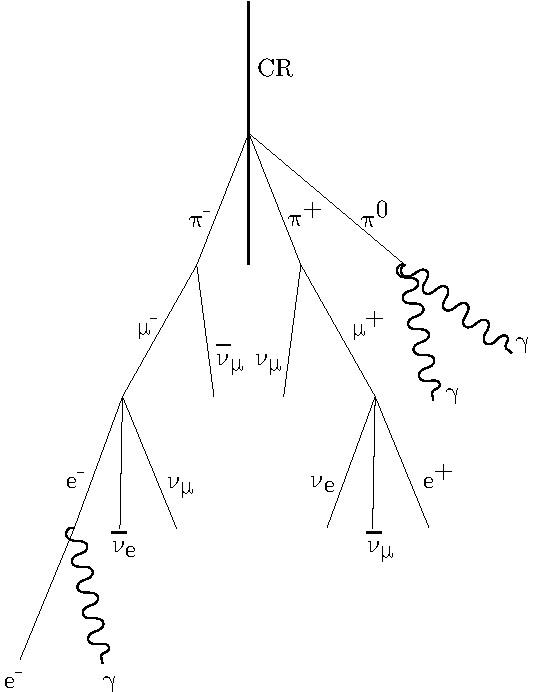
\includegraphics[width=0.5\textwidth]{05_Astronomy/Images/air_shower/cosmic_ray.pdf}
    \caption{The formation of an air shower triggered by a cosmic ray entering the atmosphere. The cosmic ray undergoes proton-proton interactions to produce neutral and charged pions. Neutral pions decay into two photons (which can trigger an electromagnetic air shower) while charged pions decay into muons and neutrinos. The muons decay into electrons/positrons and neutrinos. Depending on its energy, the original cosmic ray can undergo further proton-proton collision.}
    \label{fig:chapter_2_air_shower_hadron}
\end{SCfigure}
Both gamma rays and cosmic rays initiate air showers upon entering the atmosphere. Therefore, any observatory dedicated to studying gamma rays must be able to distinguish between a gamma-ray air shower and cosmic-ray air shower.
\newpar
Cosmic rays (protons or nucleii) above a few $\GeV$ undergo proton-proton collisions (see \autoref{sec:chapter1_hadronic_gr_emission}) with atmospheric nuclei and produce pions.

\begin{equation}
    \begin{aligned}
    \text{CR} + p_\text{atmos} &\rightarrow \text{CR} + \pionneutral + \pionminus + \pionplus
    \end{aligned}
\end{equation}

\noindent where the ratio of charged pions to neutral pions is approximately $2:1$. Charged pions decay into neutrinos and muons, with muons then decaying into electrons, positrons, neutrinos and anti-neutrinos. The presence of muons in an air shower can indicate whether the shower was triggered by a gamma ray or cosmic ray. Electrons and positrons interact with the atmosphere via Bremstrahlung and electron-positron annihilation to produce photons as discussed in \autoref{sec:05_air_shower_gamma_ray}. Unlike gamma-ray air showers, the original cosmic ray can go on to undergo further proton-proton collisions to increase the number of charged pions in the atmosphere. This development of cosmic-ray air showers is shown in \autoref{fig:chapter_2_air_shower_hadron}.
\newpar
The decay length, $d$, is defined to be the distance a particle with Lorentz factor $\gamma$ will travel before it decays \citep{MATTHEWS2005387}:

\begin{equation}
    \begin{aligned}
    d=\beta \gamma c \tau \text{ ,}
    \end{aligned}
\end{equation}
\noindent where ($\tau$ is the mean lifetime of the particle). The mean life time of charged pions is approximately $2.6\times 10^{-8}\,\si{\second}$, while neutral pions have a mean life of $8.4\times 10^{-17}\,\secs$. This gives the decay length for neutral and charged pions to be $d_{\pi_0}=\gamma \times  2.51 \times 10^{-6}\,\cm$ and $d_{\pi_\pm}= 780\gamma\,\cm$ respectively. Compared to charged pions, neutral pions decay essentially where they were created.
%Unlike Heitler's model of gamma-ray air showers, the radiation length for the decay of neutral and charged pions cannot be assumed to be identical.
\begin{SCfigure}[][h!]
    \centering
    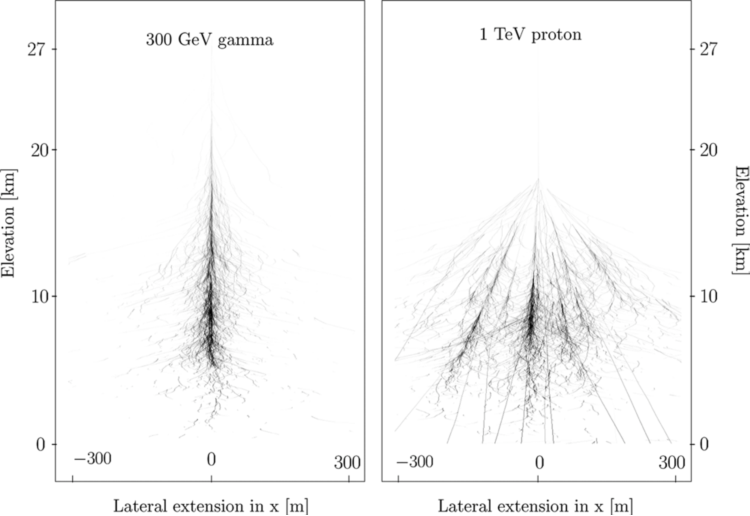
\includegraphics[width=0.7\textwidth]{05_Astronomy/Images/air_shower/cosmic_ray_vs_gamma_ray2.pdf}
    \caption{Monte Carlo simulations of a air shower triggered by a $0.3\,\TeV$ gamma ray (\textit{left}) vs an air shower triggered by a $1\,\TeV$ cosmic-ray proton (\textit{right}). Image courtesy of \cite{2008RPPh...71i6901A}}
    \label{fig:chapter_2_air_shower2}
\end{SCfigure}
\newpar 
After $n$ interactions, there are $N_{\pi_\pm}$ charged pions with individual energy \citep{MATTHEWS2005387}:

\begin{equation}
    \begin{aligned}
    E_\pi &=\frac{E_0}{(\frac{3}{2}N_\text{ch})^n}\text{ ,}
    \end{aligned}
\end{equation}
\noindent where $E_0$ is the energy of the initial cosmic ray and $N_\text{ch}$ is the multiplicity of charged particles produced in hadronic interactions.
\newpar
\cite{MATTHEWS2005387} gives the number of interactions (of the initial cosmic ray) for a pion to reach critical energy, $E_c^\pi$, to be:
\begin{equation}
    \begin{aligned}
    n_c&=\frac{\ln(E_0/E_c^\pi)}{\frac{3}{2}N_\text{ch}}=0.85\log_{10}\qty(\frac{E_0}{E_c^\pi}) \text{ ,}
    \end{aligned}
\end{equation}
\noindent occurring when the probability of pion decay exceeds the probability that it survives to the next interaction. The original energy of the cosmic ray is now divided between $N_\pi$ pions and $N_\text{max}$ electromagnetic particles:

\begin{equation}
    \begin{aligned}
    E_0&=N_\mu E_c^\pi + N_c^e N_\text{max} \\
 &\approx 0.85\,\GeV\qty(N_e+24 N_\mu)\text{ ,}
    \end{aligned}
\end{equation}
\noindent where $N_e=N_\text{max}/10$ from \autoref{eq:chapter_2_gas_e_correction_factor}
\newpar
The atmospheric depth where the number of air shower particles is at a maximum, $X_\text{max}^p$, is found through \citep{MATTHEWS2005387}:
\begin{equation}
    \begin{aligned}
    X_\text{max}^p&= X_0 + \lambda_r\ln(\frac{E_0}{3N_\text{ch}E_c^e}) =470+58\log_{10}\qty(E_0/1\,\PeV)\,\grampercentimetresquared \text{ ,}  
    \end{aligned}
\end{equation}
\noindent where $X_0$ is the atmospheric depth where the shower was initiated. The atmospheric depth maximum can be compared to the atmospheric depth maximum for gamma-ray air showers via:
\begin{equation}
    \begin{aligned}
    X_\text{max}^p=X_\text{max}^\gamma+X_0-\gamma_r\ln 3N_\text{ch}\text{ .}
    \end{aligned}
\end{equation}
\noindent This gives the elongation rate for proton initiated air showers:

\begin{equation}
    \begin{aligned}
    \Lambda^p &= \Lambda^\gamma + \dv{ }{\log_{10}E_0}\qty[X-\lambda_r\ln 3N_{ch}] \\
    &\approx 58\,\grampercentimetresquared\,\text{per decade of primary energy}\text{ .}
    \end{aligned}
\end{equation}
\noindent \autoref{fig:chapter_2_air_shower2} compares Monte Carlo simulations of air showers triggered by a $0.3\,\TeV$ gamma ray and a $1\,\TeV$ cosmic-ray proton, where the hadronic air shower is more spread out than gamma-ray air shower. Additionally, any photons produced by proton-proton interactions can trigger an electromagnetic shower within a hadronic air shower. Using this information, gamma-ray observatories can analyse the air shower to determine whether the initial particle was a gamma ray or proton.

\subsection{Cherenkov Light and Cherenkov Telescopes}

Particles produced in a electromagnetic air shower can travel faster than the speed of light in the atmosphere. The speed of light, $c_n$, in a medium with refractive index $n$ is given by:

\begin{equation}
    \begin{aligned}
    c_n = \frac{c}{n}\text{ ,}
    \end{aligned}
\end{equation}
\noindent where $c=3.0\times 10^8\,\si{\meter\per\second}$ and $n>1$.
\newpar 
A charged particle polarises the medium it is travelling through. As the particle propagates, the polarised medium oscillates back to its resting state and emits electromagnetic radiation. This is shown in \autoref{fig:chapter_2_chernkov_light}, where the resulting radiation can be described by Huygen's construction of light. For a particle that is travelling with velocity less than the speed of light, the electromagnetic radiation wave-fronts will destructively interfere with each other with no net production. If the charged particle is travelling faster than the speed of light in that medium, the electromagnetic wave-fronts will constructively interfere and there is a net production of light.
\newpar
\begin{SCfigure}[1][h!]
    % \centering
    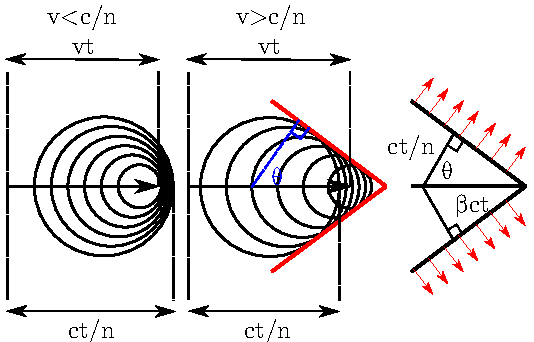
\includegraphics[width=0.5\textwidth]{05_Astronomy/Images/air_shower/chernkov_light.pdf}
    % \caption{ }
    \caption{Huygens's construction of a charged particle travelling at speed $v$ in a medium of refractive index $n$. Cherenkov light is emitted at angle $\theta$ when the particle is travelling faster than the speed of light in the medium}
    \label{fig:chapter_2_chernkov_light}
\end{SCfigure}
Cherenkov light is emitted in a cone in the direction of particle propagation (see \autoref{fig:chapter_2_chernkov_light}). At time $t=0$, a photon is emitted at angle $\theta$ to the particle propagation. After time $t$, the photon has travelled distance $ct/n$ and the particle has travelled $\beta ct$ ($\beta=v/c$, with v being the velocity of the particle). Hence:
\begin{equation}
    \begin{aligned}
    \cos\theta &= \frac{ct}{n} \frac{1}{\beta ct} \\
    &=\frac{1}{n\beta}\text{ .}
    \end{aligned}
\end{equation}
\noindent For ultra relativistic particles, $\beta\rightarrow 1$ and the light is emitted at angle $\theta \rightarrow \cos[-1](1/n)$.
\newpar
The threshold for particle with mass $m$ to produce Cherenkov light occurs when it is travelling at the speed of light in a medium $(v=c/n)$:

\begin{equation}
    \begin{aligned}
    E_\text{thr}&=\gamma mc^2=\frac{mc^2}{\sqrt{1-{1}/{n^2}}}\text{ .}
    \end{aligned}
\end{equation}
\noindent For electrons at sea level ($n=1.0003$), the threshold energy is $\approx 21\,\MeV$. In water, $n=1.33$, the threshold energy decreases to $1\,\MeV$. Observatories such as the Pierre Auger observatory and the High Altitude Water Cherenkov gamma-ray observatory use water tanks (which has a higher refractive index $n=1.33$, hence slower speed of light than air) to produce Cherenkov light \citep{alma9924446790001811}.

\begin{figure}[h]
    \centering
    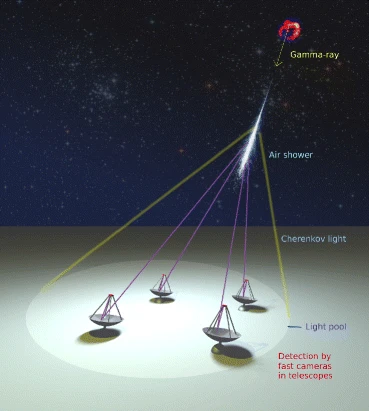
\includegraphics[height=0.4\textheight]{05_Astronomy/Images/air_shower/chenkov_light_pool.png}
    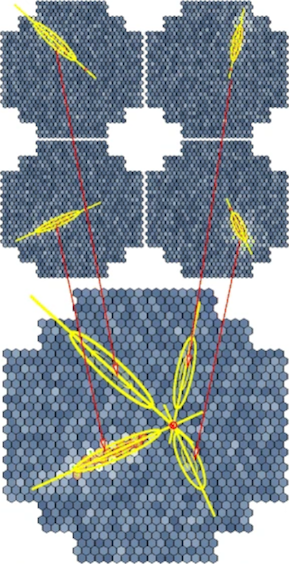
\includegraphics[height=0.4\textheight]{05_Astronomy/Images/air_shower/cherenkov_telescope.png}
    \caption{(\textit{left}) Pool of Cherenkov light from an air shower observed by four telescopes in a stereo system.
    (\textit{right}) Projection of the Cherenkov light onto one camera focal plane by the four telescopes. Images courtesy of \cite{2009ExA....25..173V,}.}
    \label{fig:chapter_2_chernkov_telescope}
\end{figure}
\newpar
The air shower forms an observable pool of Cherenkov light on the ground as shown by the left-hand panel of \autoref{fig:chapter_2_chernkov_telescope}. At sea level, the radius of the light cone is approximately $125\,\si{\meter}$ for a primary gamma ray of energy $0.1\,\TeV$ but can extend to $1\,\si{\kilo\meter}$ for energies greater than $100\,\TeV$ \citep{Patterson_1983}.  A telescope can be placed anywhere within the light pool to detect the Chernkov light produced from particles in an air shower. Hence, the the effective collection area of the telescopes becomes the area of the light pool at the ground, which is of order $\approx1\,\si{\kilo\meter\squared}$.
\newpar
The top-right hand panel of \autoref{fig:chapter_2_chernkov_telescope} shows how Cherenkov light is observed by single and multiple telescopes. To characterise Cherenkov light, the light is first modelled by an ellipse and then parameters such as the width, length, location \& azimuthal angle to the center of the telescope is found. These parameters, known as the Hillas parameters \citep{1985ICRC....3..445H}, can be used to determine the arrival direction, energy and type of the particle that triggered the air shower. If multiple telescopes observe the same light at different angles, the combined image (see the right hand panel of \autoref{fig:chapter_2_chernkov_telescope}) can be reconstructed using `stereo' techniques with far more precision than if one telescope was used.

\section{TeV Gamma-Ray Observatories} \label{sec:02_TeV_observatories}

Evidence of $\TeV$ gamma rays from AGN Centaurus were reported by \cite{1975ApJ...197L...9G}. But $\TeV$ astronomy effectively began with the detection of TeV gamma rays from the Crab Nebula \citep{1989ApJ...342..379W}. Over three decades later, $\TeV$ gamma rays from over 200 sources have been detected \citep{2008ICRC....3.1341W}. This section will describe some of the $\TeV$ gamma-ray observatories whose data pata products were used in this thesis.

\subsection{The High Energy Stereoscopic System} \label{sec:02_HESS}

\begin{figure}[h]
    \centering
    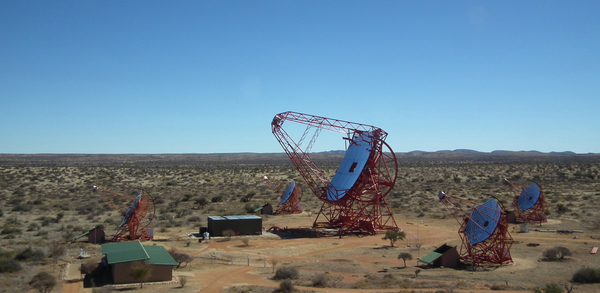
\includegraphics[width=\textwidth]{05_Astronomy/Images/telescopes/HESS_image.jpg}
    \caption{The High Energy Stereoscopic System. Images from \citep{HESS}.}
    \label{fig:chapter_2_HESS}
\end{figure}
\begin{figure}[h]
    \centering
    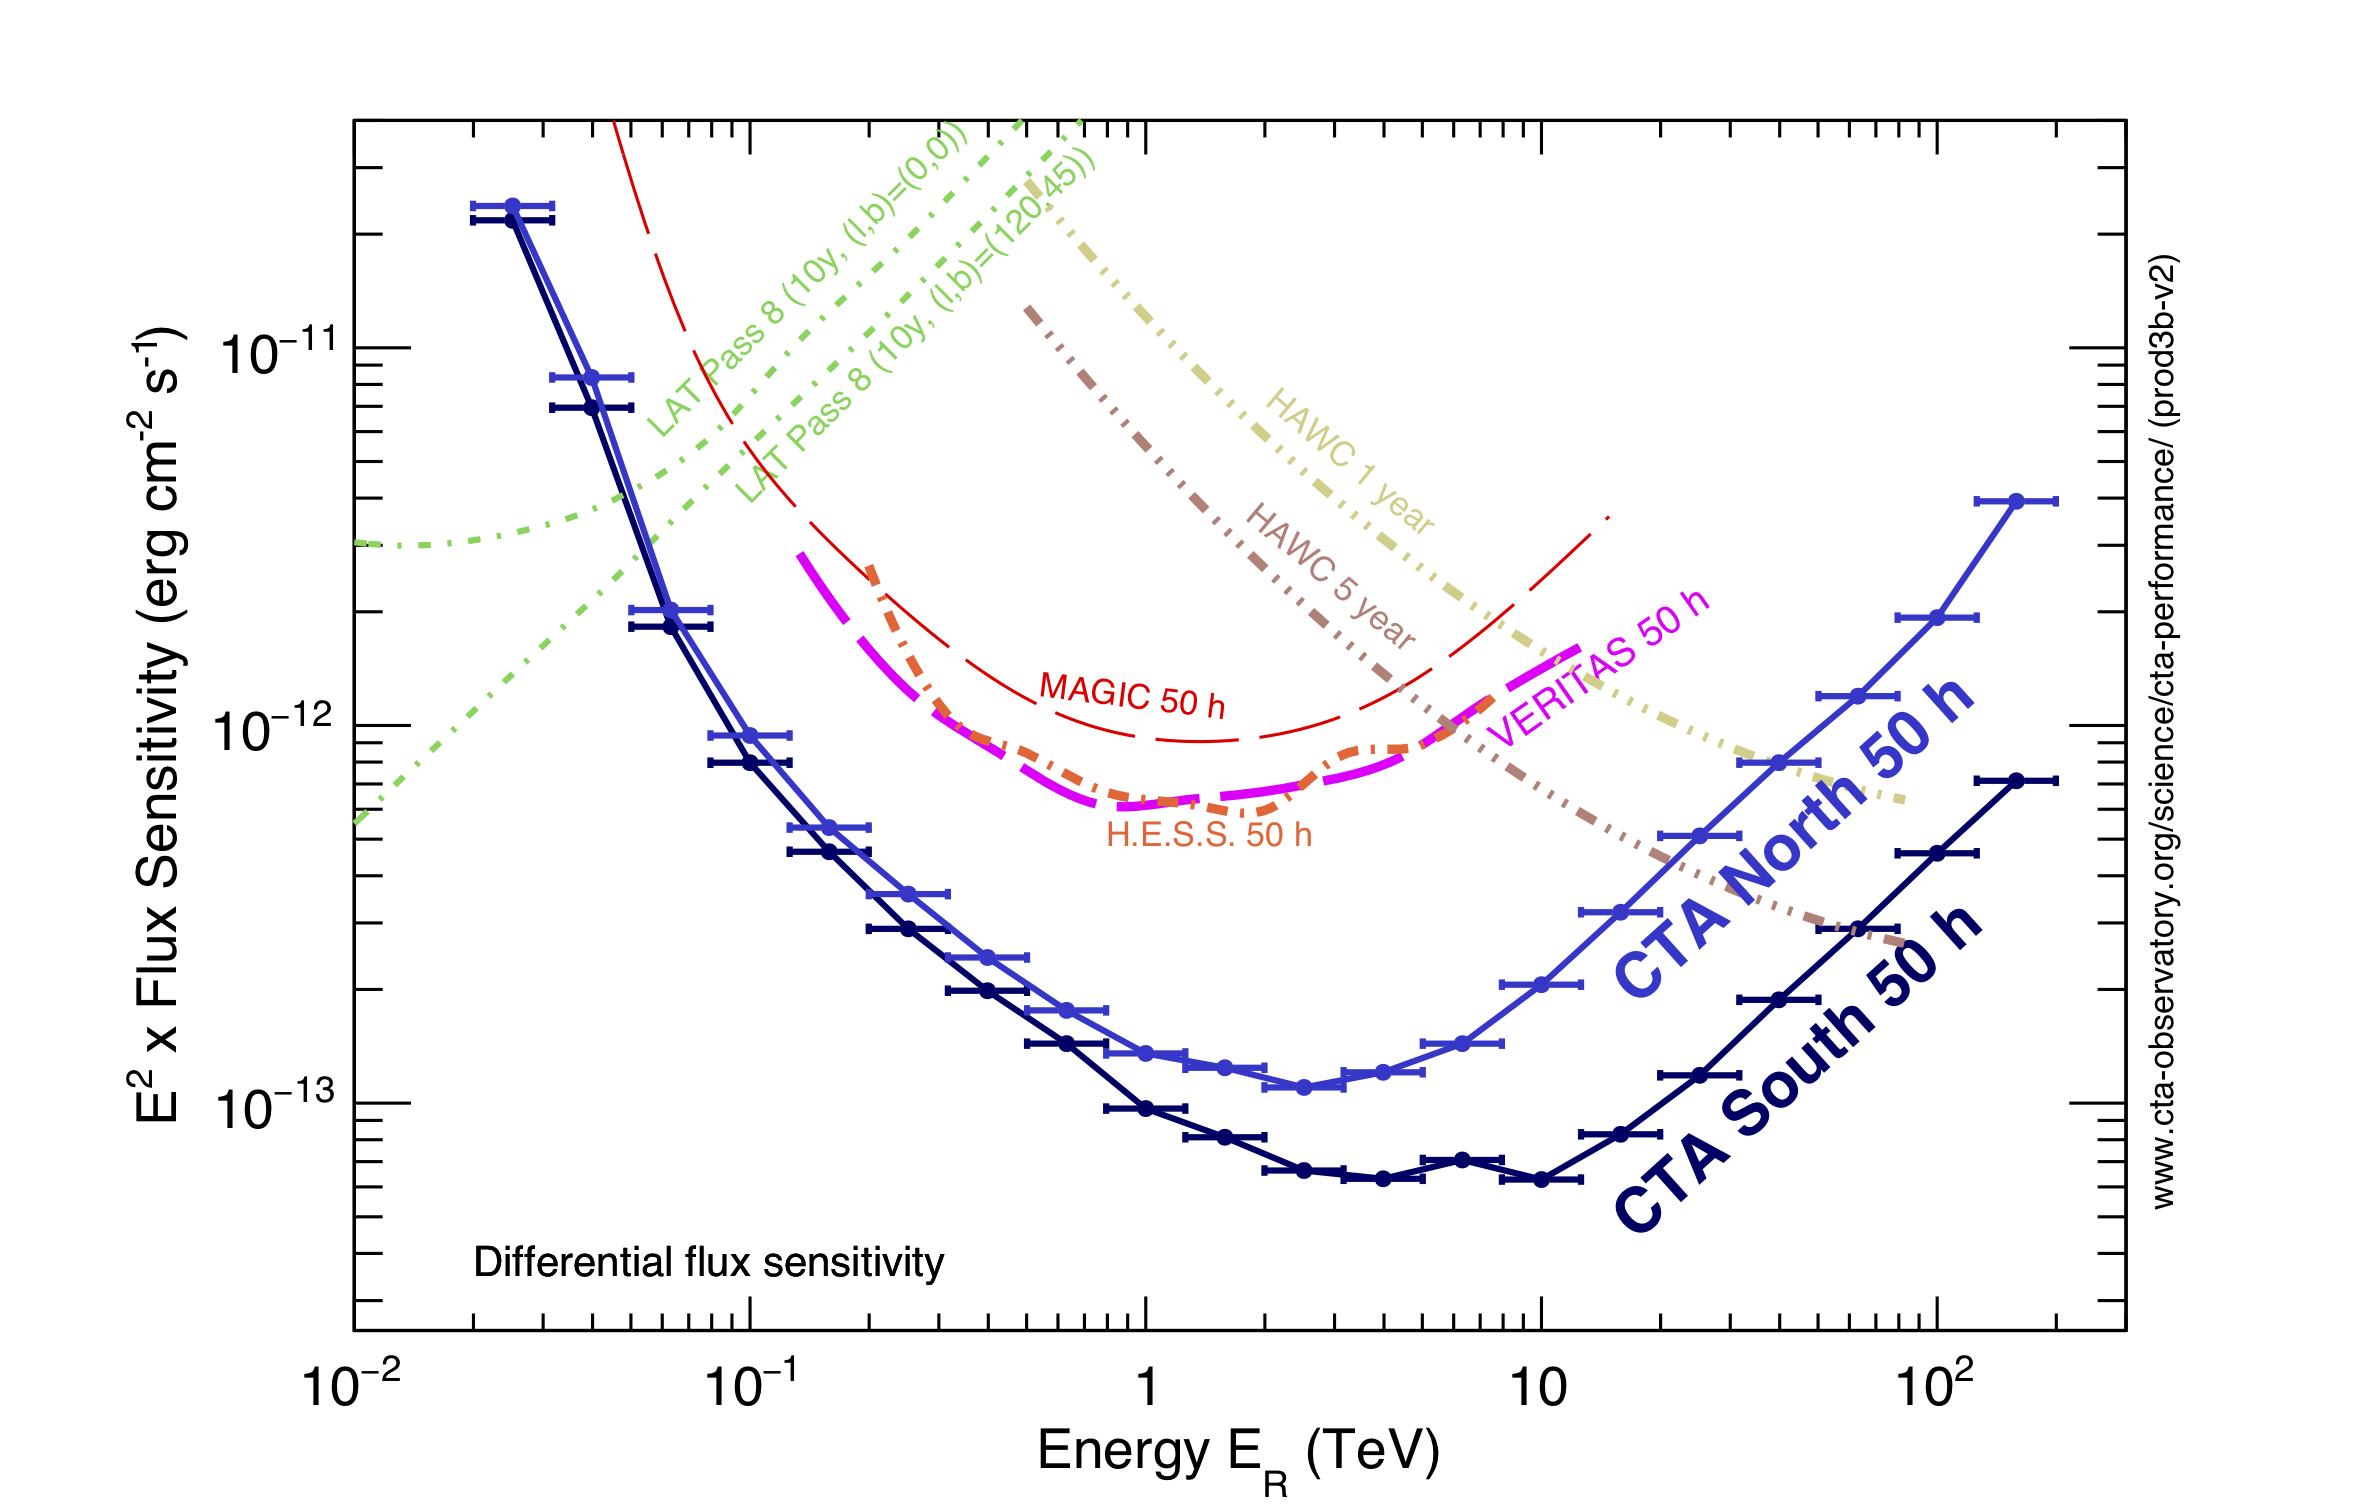
\includegraphics[width=0.9\textwidth]{05_Astronomy/Images/telescopes/sensitivity_comparison.png}
    \caption{Comparison of the performance (minimum detectable flux) of different gamma-ray instruments for an observation time of $50\,\si{h}$. H.E.S.S., CTA south and CTA north is shown by the red, dark blue and light blue lines respectively. Image courtesy of \cite{2019scta.book.....C}.}
    \label{fig:chapter_2_sensitivity comparison}
\end{figure}

The High Energy Stereoscopic System (H.E.S.S.) telescope (named after Victor Hess) is an array of telescopes located at $1800\,\si{\m}$ above sea lebvel in Namibia (see \autoref{fig:chapter_2_HESS}) \citep{HESS}. H.E.S.S. consists of five telescopes and utilises the atmospheric Cherenkov imaging technique described above to detect gamma radiation in the energy range $20\,\GeV$ to $100\,\TeV$. A comparison of the performance of H.E.S.S. to other instruments is shown in \autoref{fig:chapter_2_sensitivity comparison}. The angular resolution of H.E.S.S. ($\leq\ang{0.1}$) allows detailed observations of gamma-ray sources, which is key in understanding the morphology of objects such as SNRs and PWNe \citep{2018A&A...612A...1H}. HESS was constructed in two different phases; Phase I consisting of four $12\,\m$ telescopes and Phase II added one $28\,\m$ telescope at the centre of the array. Phase I and Phase II of H.E.S.S. commenced operations in December 2003 and July 2012 respectively. 
\newpar 
The four $12\,\m$ telescopes of Phase I have 382 mirror segments of $0.6\,\m$ diameter mounted onto a steel frame in a Davies-Cotton optical layout (a parabolic layout where each mirror has focal length $f$, which is the focal length of the entire telescope ($15\,\m$)) \citep{2003APh....20..111B}. The mirrors combine to have total mirror surface area of $107\,\si{\meter\squared}$ and focus the Cherenkov light onto a photomultiplier camera (containing $\approx 1000$ pixels) with a $\ang{5}$ field of view. Each dish is mounted on a rotating base frame which rotates azimuthally on a rail of $13.6\,\m$ diameter. The telescopes have a peak positioning speed of $100\si{^\circ\per\minute}$ in both azimuth and elevation and is sensitive to gamma rays above $100\,\GeV$. This is ideal for observing events such as gamma-ray bursts and following up activity triggered by other observatories (e.g. neutrinos from IceCube, GRBs from Swift). The four telescopes are placed in a square geometry with distances $120\,\m$ from each other.
\newpar
Phase II of H.E.S.S. placed an additional $24\,\m$ telescope in the centre of phase I \citep{2005ICRC....5..163V}. The telescope consists of 875 hexagonal mirrors of $0.9\,\m$ sides laid out in a parabolic shape with focal length of $36\,\m$ and total mirror area of $614\,\si{\meter\squared}$. The Phase II telescope has azimuth and elevation speed of $200\si{^\circ\per\minute}$ and $100\si{^\circ\per\minute}$ respectively. Similar to Phase I, Phase II focuses Cherenkov light onto a photomultiplier camera consisting of $\approx 2000$ pixels with a $\ang{3.2}$ view of the sky.

\subsubsection{The H.E.S.S. Galactic Plane Survey}

\begin{figure}[h]
    \centering
    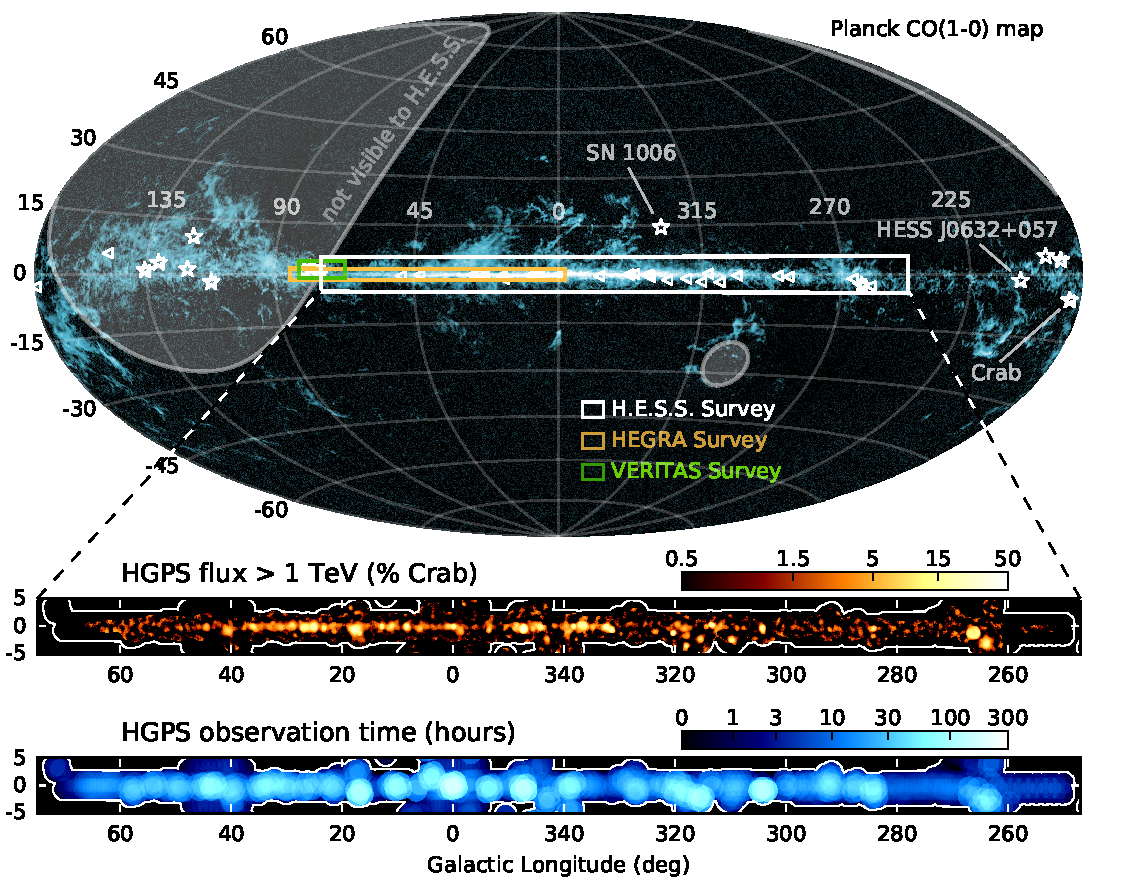
\includegraphics[width=0.9\textwidth]{05_Astronomy/Images/telescopes/hess_survey.pdf}
    \caption{The H.E.S.S. Galactic plane survey superimposed onto \textit{Planck} CO data. Image courtesy of \cite{2018A&A...612A...1H}.}
    \label{fig:chapter_2_HESS_survey}
\end{figure}

In 2018, H.E.S.S. released its third Galactic Plane Survey (HGPS) in $\TeV$ gamma rays that covers data from January 2004 to January 2013 totalling $2864\si{\hour}$ of observation time \citep{2018A&A...612A...1H}. The HGPS catalogued 78 very high energy (VHE) sources compared to 10 sources in the first release \citep{2005Sci...307.1938A} and  22 in its second \citep{2006ApJ...636..777A}. Of the 78 VHE sources; 3 are binary objects (composed of a massive star and a compact object), 8 are SNRs, 12 are PWN, 8 are composite objects (SNR + PWN), 11 have no known association and a further 36 are not firmly identified. \cite{2018A&A...612A...1H} found that 47 of the HGPS sources ($60\%$) had an associated pulsar and ($39\%$ being a PWN or a composite object (SNR + PWN). This makes PWNe the largest source class in the survey. Following the HPGS survey, \cite{2018A&A...612A...2H} conducted a study on the population of $\TeV$ PWN to link PWN evolutionary theory to $\TeV$ observations (see \autoref{sec:01_PWN_TeVPWN} for further detail). This thesis focuses on the $\TeV$ PWN \mbox{HESS\,J1825-137}.

\subsection{\textit{Fermi}-LAT}

The \textit{Fermi} Gamma-ray Space Telescope is a space based observatory launched on the 11th of June 2008. \textit{Fermi} has two instruments; the Large Area Telescope (LAT) and the Gamma-ray Burst Monitor \citep{2010RPPh...73g4901M}. \textit{Fermi}-LAT consists of thin metal sheets that assist in the production of electron-positron pairs. The electron-positron pair then pass through microstrip detectors that can track their trajectory. Finally, the products enter a calorimeter which measures the combined energy of the electron-positron pair to determine the energy of the initial gamma ray. The Gamma-ray Burst Monitor consists of scintillators positioned on opposite sides of the spacecraft allowing different viewing angles to detect gamma-ray bursts and solar flares \citep{2010RPPh...73g4901M}. The performance characteristic of \textit{Fermi}-LAT allows sensitivity in the energy range of $20\,\MeV - 300\,\GeV$ with a field of view of $2.4\,\si{\steradian}$ \citep{2010RPPh...73g4901M}. 
\newpar
The equivalent \textit{Fermi}-LAT source towards \mbox{HESS\,J1825-137} is \mbox{4FGL\,J1824.5\,1351e} \citep{2020ApJS..247...33A}. \cite{2020A&A...640A..76P} combined GeV data from \textit{Fermi}-LAT and $\TeV$ data from H.E.S.S. to provide a broader view of the gamma-ray emission towards \mbox{HESS\,J1825-137} from $1\,\GeV$ up to $100\,\TeV$. They found that the size of the PWN increases at lower energies, implying that electrons from the outer edges are from an older population of electrons compared to the recently injected electrons near the powering pulsar. This is indicative of a $\TeV$ halo forming, where electrons begin to escape the PWN into the ISM and emit $\TeV$ emission via inverse Compton interactions.

\subsection{LHAASO}

The Large High Altitude Air Shower Observatory (LHAASO) is a gamma-ray and cosmic-ray observatory located $\approx 4400\,\m$ above sea level in Sichuan China \citep{2022ChPhC..46c0001M}. LHAASO consists of:
\begin{figure}[h!]
    \centering
    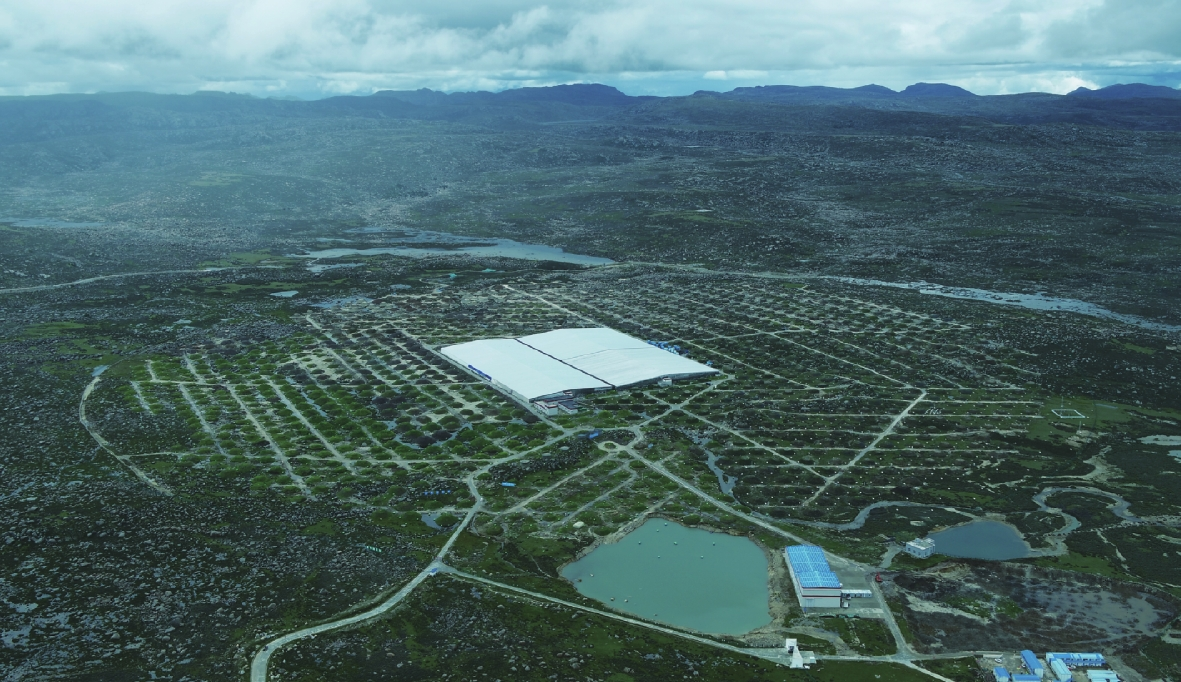
\includegraphics[height=0.15\textheight]{05_Astronomy/Images/telescopes/LHAASO.jpg}
    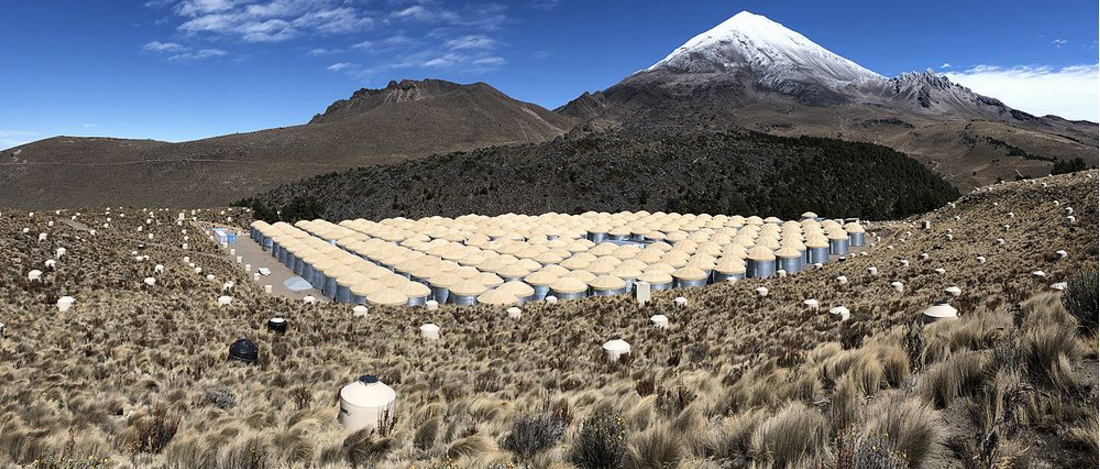
\includegraphics[height=0.15\textheight]{05_Astronomy/Images/telescopes/HAWC.png}
    \caption{The LHAASO (\textit{left}) and HAWC (\textit{right}) observatories. Images courtesy of \cite{2022ChPhC..46c0001M} and \cite{2023NIMPA105268253A}}
    \label{fig:my_label}
\end{figure}
\begin{itemize}
    \itemsep0em
    \item $1.3\,\si{\kilo\meter\squared}$ array of $\approx 5200$ electromagnetic detectors and muon detectors that focuses on detecting gamma rays above $30\,\TeV$ and cosmic rays from $10\,\TeV$ to $100\,\PeV$ \citep{2021ChPhC..45b5002A}.
    \item A water Cherenkov array sensitive to gamma rays between $100\,\GeV$ and $30\,\TeV$ and has total detection area of $7.8\times 10^4\,\si{\meter\squared}$. This array monitors galactic gamma-ray sources, gamma-ray bursts and AGNs \citep{2021arXiv210103508L}.
    \item 18 Cherenkov telescopes that aims to measure the cosmic-ray energy spectrum and composition between $10\,\TeV$ and $1\,\si{E\electronvolt}$ \citep{2021EPJC...81..657A}.
    \item An upcoming electron-neutron detector array to study the cosmic-ray spectrum and composition above $1\,\PeV$ \citep{2022ChPhC..46c0001M}.
\end{itemize}
\newpar
LHAASO has detected significant gamma-ray emission above $100\,\TeV$ from 12 Galactic sources including \mbox{LHAASO\,1825-1326} (LHAASO equivalent of \mbox{HESS\,J1825-137} / \mbox{HESS\,J1826-130}, see \autoref{fig:chapter1_hess_j1825_137_object_positions}) \citep{2021Natur.594...33C}. In 2021, LHAASO revealed the detection of gamma rays up to $1.1\,\PeV$ from the Crab Nebula, implying the existence of a $2.3\,\PeV$ electron \citep{doi:10.1126/science.abg5137}

\subsection{HAWC}

The High Altitude Water Cherenkov Observatory (HAWC) is a gamma-ray and cosmic-ray observatory located in Puebla, Mexico. The primary detector of HAWC consists of $300$ water tanks arranged in a $22\,000\,\si{\meter\squared}$ area at an altitude of $\approx 4100\,\m$ above sea level \citep{2023NIMPA105268253A}. The high refractive index of water ($n=1.33$) lowers the cosmic-ray/gamma-ray energy threshold to produce Cherenkov light which is then observed by four photomultiplier tubes.
\newpar
HAWC has detected over $100$ sources of VHE gamma rays, which are summarised in the third HAWC catalogue \citep{2020ApJ...905...76A}. \cite{PhysRevLett.124.021102} revealed $9$ gamma-ray sources with emission above $56\,\TeV$, with three of these sources having significant detection above $100\,\TeV$. This includes the equivalent \mbox{HESS\,J1825-137} / \mbox{HESS\,J1826-130}: \mbox{eHWC\,J1825-134}.

\subsection{The Cherenkov Telescope Array}

\begin{figure}[ht]
    \centering
    \includegraphics[width=0.9\textwidth]{05_Astronomy/Images/telescopes/cta_image.jpg}
    \caption{Telescopes for the Cherenkov Telescope Array. From left to right: the Small-Sized Telescope, two of the proposed Middle-Sized Telescope and the Large-Size Telescope. Image courtesy of \cite{cherenkov_telescope_array}.}
    \label{fig:chapter_2_cta}
\end{figure}

The Cherenkov Telescope Array (CTA) is the next generation ground-based telescope array that will observe gamma rays from $10\,\GeV$ up to $300\,\TeV$. It will be the largest ground-based telescope that can observe the night sky with sensitivity up to $10$ times greater than current instruments (see \autoref{fig:chapter_2_sensitivity comparison}). CTA will have two arrays in both the Southern (Chile) and Northern hemisphere (Canary Islands) to allow access to the majority of the night sky.
\newpar
CTA will be an array of three different sized telescopes (see \autoref{fig:chapter_2_cta}): Small-Sized Telescopes (sensitive to energies $>1\,\TeV$) with a mirror diameter and field of view of $4\,\m$ and $\approx\ang{0}$ respectively, Medium-Sized Telescopes (sensitive to energies between $80\,\GeV$ and $50\,\TeV$) with a mirror diameter and field of view of $11.5\,\m$ and $\approx\ang{7.5}$ respectively and the Large-Sized Telescope (sensitive to the lowest energy gamma rays) with a mirror diameter and field of view of $\approx 23\,\m$ and $\approx\ang{4.3}$ respectively \citep{cherenkov_telescope_array,2019scta.book.....C}.
\newpar
PWN transitioning from their second to their third stage of evolution (see \autoref{sec:01_intro_time_ev_PWN}) are too faint and/or extended for their emission to be detected by current instruments such as H.E.S.S.. The increased sensitivity of CTA (see \autoref{fig:chapter_2_sensitivity comparison}) will be able observe these previously undetectable $\TeV$ PWN, providing more insight into the evolution of PWN.